Cette partie détaillera la réalisation technique du logiciel Project3Donuts.

\subsubsection{Présentation générale de la réalisation}
\paragraph{}
La partie Réalisation de ce projet se sera étalée sur les mois de Décembre, Janvier, Février et Mars. Grâce à la réflexion effectuée durant la phase de rédaction du cahier des charges, nous avons pu aborder notre projet avec une idée claire des priorités.

\paragraph{}
L'implémentation des algorithmes de rendus étant centrale au projet, nous avons dès le début de la réalisation mis en place deux équipes de deux personnes pour les deux rendus principaux : les anaglyphes et les autostéréogrammes. Les folioscopes quand à eux ne demandaient pas d'algorithmes particulier, si ce n'est la manipulation de la caméra vis à vis de la scène qui allait être mise en place grâce à la troisième équipe.

\paragraph{}
Le travail sur la scène s'est basé sur le prototype généré lors de la phase du cahier des charges. Il a ainsi été amélioré pour intégrer les parseurs de fichiers objets qui allaient être nécessaires pour la génération des éléments de la scène, et rendre plus agrèable la manipulation des objets et les déplacements dans la scène.

\paragraph{}
Malheureusement, l'implémentation des algorithmes s'est révélée plus longue que nous l'avions initialement prévue. Le mois prévisionnel n'étant pas uniquement dédié au projet PFA, les différents imprévus et une sous-estimation de la difficulté que représentait cette étape ont engendré un retard par rapport au prévision. De plus amples explications seront données dans la partie ``Difficultés rencontrées'' de ce rapport. 
Au final, les recherches et implémentations concernant les autostéréogrammes et anaglyphes auront pris deux mois et demi au lieu d'un seul. Deux mois ont servi à la réalisation de tests sur des prototypes pour évaluer la qualité des rendus, le demi-mois restant concerne l'intégration au reste du logiciel avec d'autres tests pour trouver les réglages optimaux des algorithmes.

\paragraph{}
En parallèle, la troisième équipe, appuyée parfois par des membres des autres groupes en cas de besoin, a continué d'avancer sur la partie Scène du logiciel. L'implémentation de certaines manipulations de scène (déplacements de la caméra ou des objets notamment) auront parfois étaient plus rapides que prévu, mêmes si quelques retours en arrière ont été nécessaires au milieu du projet comme nous l'expliquerons dans la partie ``Difficultés rencontrées''.

L'ordre chronologique initialement prévu dans le diagramme de Gantt n'aura finalement pas toujours été respecté. Par exemple, puisqu'il était facile d'intégrer plusieurs objets dans la scène à partir de l'ajout d'un seul objet, ces deux parties auront été effectuées simultanément. Il en est de même pour la sauvegarde automatique qui aura été ajoutée en même temps que la sauvegarde classique de la scène, ou encore pour les manipulations de la scène et de l'objet dont l'implémentation était grandement facilitée par l'utilisation de la bibliothèque OpenGL pour Qt.

\paragraph{}
Au final, la totalité des tâches prévues jusqu'au début du mois de Mars auront pu être effectuées dans les temps, nous laissant le mois de Mars pour l'intégration des algorithmes au logiciel, l'amélioration de certaines fonctionnalités, le développement de l'interface et la rédaction de ce rapport.



\subsubsection{Les algorithmes du logiciel}
\paragraph{}
Pour pouvoir permettre à l'utilisateur de notre logiciel d'obtenir des anaglyphes ou des autostéréogrammes il a fallu prospecter sur Internet afin de trouver suffisamment d'articles scientifiques et de sites traitant le sujet pour établir des comparaisons et choisir parmi toutes les solutions proposées celles qui offraient le meilleur résultat.

\paragraph{}
Cet exercice s'est révélé assez complexe car le travail de recherche qui s'y rapporte a été long, et il était parfois difficile de trouver les bonnes informations pour répondre à nos interrogations. Nos clients nous auront longuement accompagné dans notre travail de recherche, et nous auront conseillé sur des outils pour trouver des articles pertinants. Cette partie ``Recherche de l'existant'', qui s'est principalement déroulée durant la phase de rédaction du cahier des charges, aura été formatrice car elle nous aura appris à utiliser les bons outils (comme google scholar\footnotemark) et les bons mots-clés pour rendre nos recherches fructueuses.
\footnotetext{\url{http://scholar.google.fr/schhp?hl=fr}}
\paragraph{}
Une fois les algorithmes choisis, l'utilisation de cartes de profondeurs et de paires d'images stéréoscopiques trouvées sur Internet ont permis de faire des tests sur des prototypes indépendants du logiciel final. Leur implémentation s'est faite durant le dernier mois du projet. Il a donc fallu définir les entrées et les sorties pour chaque méthode, afin de satisfaire l'architecture du projet et de faciliter par la suite l'intégration d'autres algorithmes dans le logiciel.
La partie gérant la scène est considérée comme une boite noire avec laquelle les algorithmes de rendus intéragissent. Seules les entrées et les sorties sont connues ce qui permet de garantir la modularité de la partie Rendu. 

\paragraph{}
Malgré les tests de pré-intégration faits sur les prototypes, des problèmes ont été rencontrés au moment de l'implémentation. Par exemple, pour les anaglyphes, le passage à l'utilisation de prises de vues issues de scènes non-réelles donnait des résultats de moins bonne qualité. Trouver le bon angle pour les couples d'images stéréoscopiques n'était pas non plus une chose aisée.
Ce problème ne provenait finalement pas de l'algorithme en lui-même, mais de la scène utilisée. En effet, les tests effectués sur des images n'avaient pas de contours aussi nets que les objets de la scène, et le rendu obtenu était correct. Toutefois, les fichiers d'extension OBJ et PLY sont constitués de triangles, et leurs bords sont très marqués, ce qui cause parfois une erreur au moment de la génération de l'anaglyphe. Une solution possible pour régler ce problème aurait été de rendre les contours des objets moins abruptes, mais cette solution n'a pas été implémentée dans notre logiciel.

\paragraph{}
Pour chacun des rendus, l'utilisateur a la possibilité de prévisualiser ce qu'il souhaite obtenir. Il peut également choisir de récupérer les rendus intermédiaires qui ont permis la génération des anaglyphes ou des autostéréogrammes, c'est-à-dire respectivement les vues stéréoscopiques gauche ou droite ou les cartes des profondeurs comme le montre la figure \ref{fig:depthLogiciel}.

\begin{figure}[h]
	\centering
	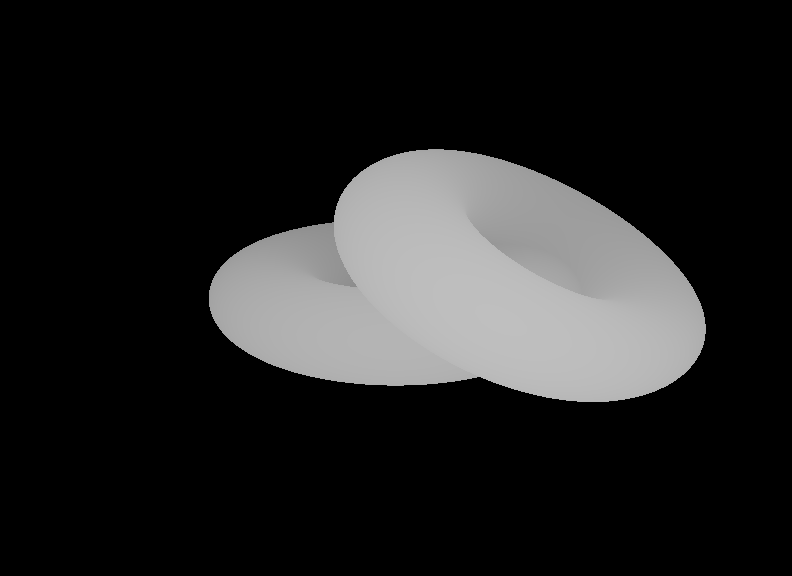
\includegraphics[scale=0.4]{depth_logiciel.png}
	\caption{\label{fig:depthLogiciel} Carte des profondeurs permettant d'obtenir un autostéréogramme \protect}
\end{figure}

\paragraph{}
Seuls les folioscopes ne proposent pas de prévisualisation avant l'enregistrement. Toutefois, ils proposent eux aussi d'enregistrer soit un GIF animé, soit l'ensemble des vues isolées, comme celles montrées dans la figure \ref{fig:flipbook_logiciel}.

\begin{figure}[h]
	\centering
	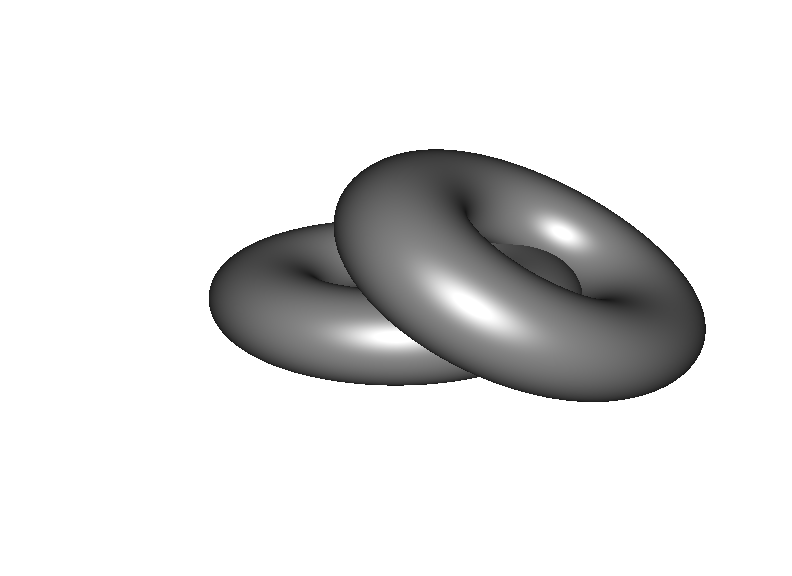
\includegraphics[scale=0.3]{testGif1.png}
        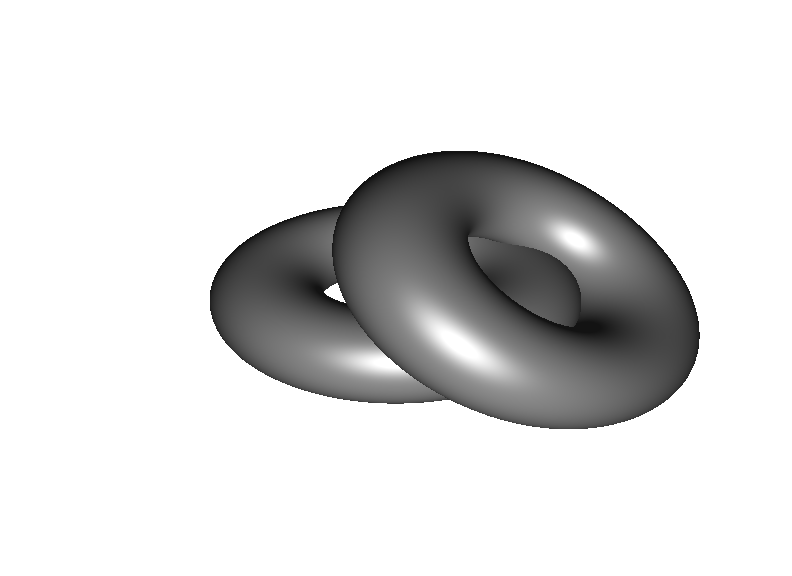
\includegraphics[scale=0.3]{testGif3.png}
        \newline
        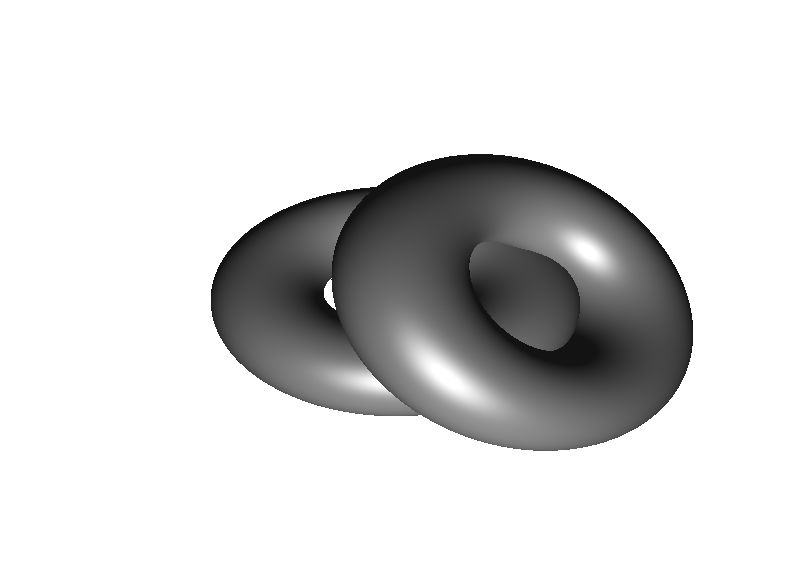
\includegraphics[scale=0.3]{testGif5.png}
        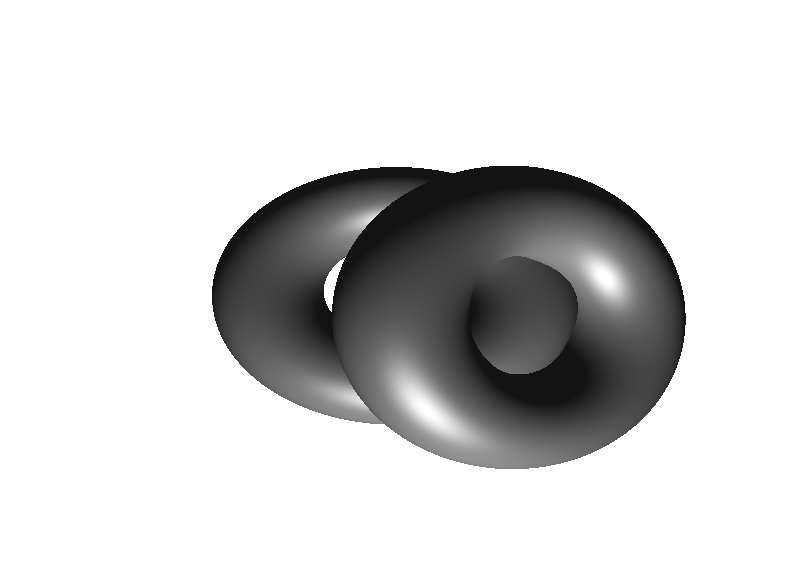
\includegraphics[scale=0.3]{testGif8.png}
	\caption{\label{fig:flipbook_logiciel} Différentes vues d'un flipbook obtenu grâce au logiciel \protect}
\end{figure}

\paragraph{}
Au final, le travail sur les algorithmes fut très enrichissant car bien plus théorique que les autres parties du projet. La recherche et la compréhension des articles est une part plus importante du travail que leur intégration au projet, d'autant plus que tous les articles ne présentaient pas dans le détail leurs solutions, ce qui obligeait à faire des recherches supplémentaires pour trouver comment s'y prendre. L'obtention d'un rendu à partir de la scène est montré dans la figure \ref{fig:screenRendu}.

\begin{figure}[h]
	\centering
	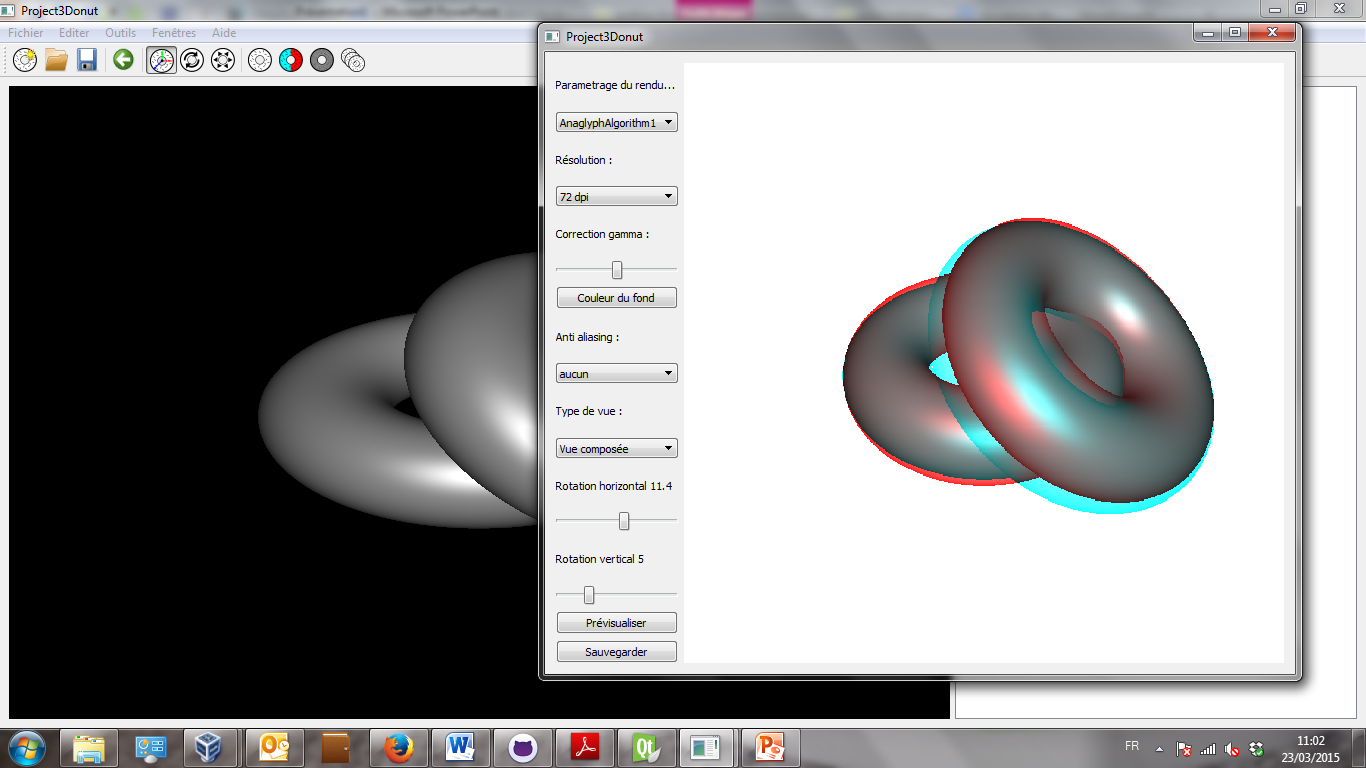
\includegraphics[scale=0.4]{rendu.png}
	\caption{\label{fig:screenRendu} Obtention d'un anaglyphe dans le logiciel \protect}
\end{figure}

\subsubsection{La manipulation de la scène}
\paragraph{}
Grâce à la rédaction du cahier des charges, les notions de scène en trois dimensions, de caméra et d'objet avaient été acquises par notre équipe avant la phase d'implémentation. Un premier prototype de la scène, présenté dans la partie Cahier des charges, aura permis une première manipulation de ces notions et des bibliothèques Qt et OpenGL pour Qt afin de créer une première scène constituée d'un seul objet. Les manipulations premières de la scène, notamment la rotation de la caméra tout autour de la scène, auront ainsi été mises en place pour pouvoir juger des capacités des bibliothèques, et déterminer la faisabilité de nos objectifs.

\paragraph{}
Dès la fin du cahier des charges, la scène aura été grandement modifiée. Les parseurs auront été finalisés pour pouvoir charger l'ensemble des fichiers objets demandés par les clients, et le stockage des objets de la scène aura été implémenté de telle façon que la gestion de plusieurs objets dans la scène a directement été opérationnelle. 

D'autres fonctionnalités, relatives à la scène et demandées par le cahier des charges, ont été implémentées peu à peu au cours de la phase de réalisation du projet. Au niveau de la scène, les rotations autour de la scène sont toujours possibles, ainsi qu'une fonction de zoom pour s'approcher ou se reculer de la scène. Au niveau des objets, la sélection d'un objet est possible soit en cliquant directement sur l'objet avec le bouton droit de la souris, soit en le sélectionnant dans la liste des objets donnée sur la fenêtre principale du logiciel. Une fois un objet choisi, on peut le déplacer, le faire tourner, modifier sa taille, sa couleur, ou encore le supprimer.

Dans les derniers temps de notre projet, nous avons pu améliorer notre scène, en permettant une translation de la caméra et en installant un repère fixe dans la scène afin que l'utilisation, malgré des rotations, puisse se repérer dans l'espace. Nous avons égalemet pu implémenter la fonctionnalité d'annulation qui permet de revenir en arrière s'il y a modification d'un objet, et ce grâce à des lambda-expressions disponibles sous C++11.

\paragraph{}
Grâce à l'ensemble des manipulations à mettre en place sur la scène, notre équipe a pu se familiariser et apprendre à utiliser les bibliothèques Qt et OpenGL pour Qt. De plus, la communauté Internet de la bibliothèque Qt nous aura été fort utile car elle aura permis de trouver des réponses à d'éventuels problèmes rencontrés, voire de poser des questions dans des cas particuliers.

\paragraph{}
La fenêtre principale du logiciel est montrée dans la figure \ref{fig:screenScene}.

\begin{figure}[h]
	\centering
	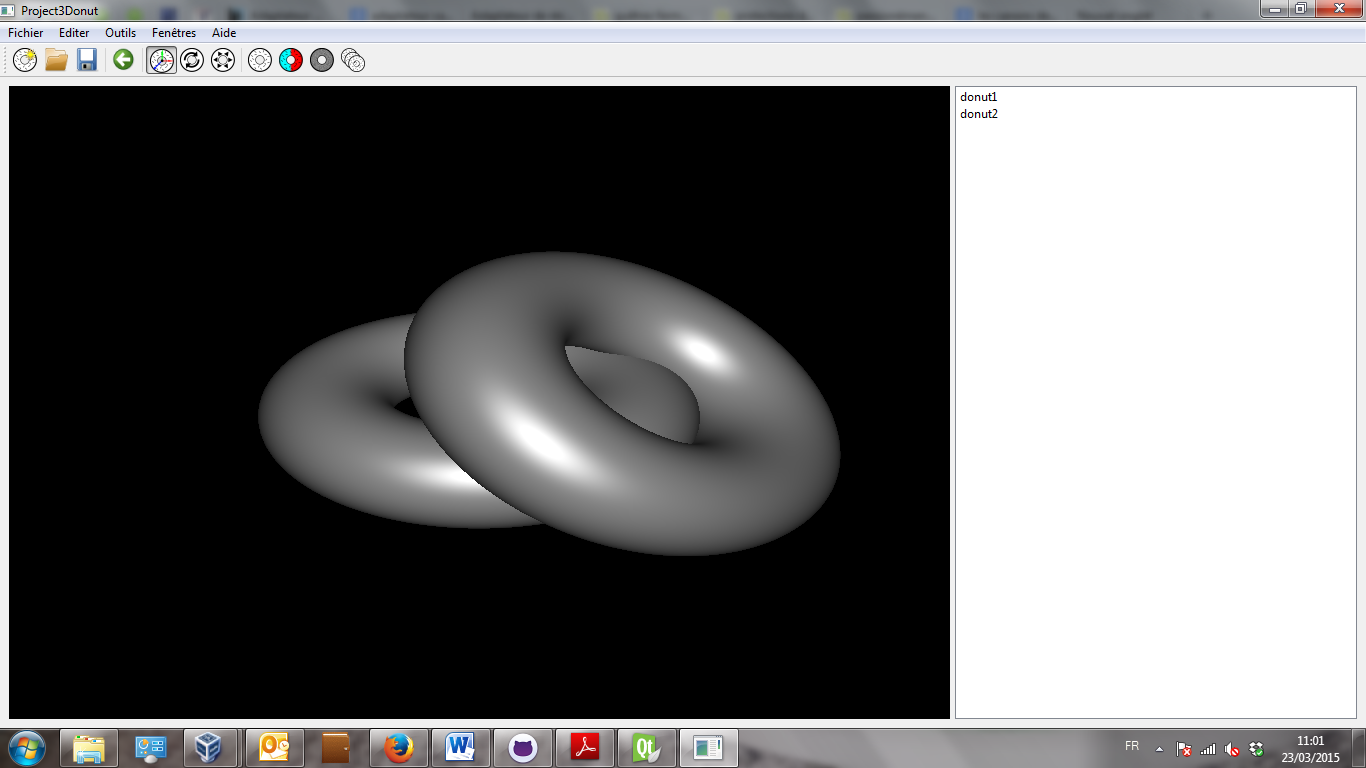
\includegraphics[scale=0.4]{Scene.png}
	\caption{\label{fig:screenScene} Visualisation de la scène dans le logiciel \protect}
\end{figure}

\subsubsection{Les sauvegardes et chargement de la scène}
\paragraph{}
Pour satisfaire la portabilité du logiciel, le nombre de bibliothèques utilisées devait être le plus faible possible. Fort heureusement, la bibliothèque Qt, portable sur la plupart des plateformes, propose une grande quantité de fonctionnalités, y compris le module QtXml qui permet la lecture et le découpage d'un fichier XML. Au cours de la phase de rédaction du Cahier des charges, nous avions mis au point un prototype de fichier XML pour permettre la sauvegarde et le chargement de la scène, que nous avons pu utiliser comme nous l'avions prévu grâce à Qt. Un exemple de fichier utilisé pour le chargement d'une scène effective dans notre logiciel, nommé 'MaScene.xml', est donné en Annexe.

\paragraph{}
La sauvegarde d'une scène consiste principalement à écrire dans un fichier texte, en respectant le format souhaité par le modèle XML, et en récupérant les bonnes informations des Objets et de la Caméra de la scène. Toutefois, deux types de sauvegarde ont été mises en place : une sauvegarde manuelle et une sauvegarde automatique.

La sauvegarde manuelle s'effectue de la même façon que dans la plupart des logiciels. A la demande de l'utilisateur, le logiciel va lancer une sauvegarde dans un fichier dont le nom est donné, et une fois que celle-ci sera achevée l'utilisateur pourra recommencer à travailler sur sa scène.

Pour la deuxième sauvegarde, nous avons dû utiliser nos connaissances acquises au cours des enseignements de Programmation Système et de Système d'Exploitation. Nous avons en effet vu d'une part comment utiliser des Threads, et d'autre part qu'un Thread en train de dormir ne demande pas d'intervention du processeur. Nous avons ainsi mis en place la création d'un Thread dès l'ajout d'un premier objet dans une scène, qui va dormir durant un certain temps avant d'effectuer une sauvegarde automatique puis de se rendormir. Cette attente passive permet ainsi de ne pas gaspiller de temps du processeur, et de conserver les avancées de la scène en cas d'arrêt non souhaité du logiciel. De plus, le temps d'attente entre deux sauvegardes automatiques peut être choisi par l'utilisateur grâce aux paramètres du logiciel.

\paragraph{}
La difficulté principale du chargement de la scène est de s'assurer de la validité du fichier XML passé en paramètre. Ainsi, de nombreuses vérifications, au fur et à mesure de la lecture du fichier, sont nécessaires afin de pouvoir créer une scène fonctionnelle. La bibliothèque QtXml aura été assez simple d'utilisation, et le chargement aura donc pu être rapidement mis en place, tout d'abord en parallèle du projet pour s'assurer que seuls les fichiers XML valides sont acceptés, puis après intégration pour s'assurer de l'appel des constructeurs et de la génération de la scène souhaitée.

\paragraph{}
L'utilisation du module QtXMl aura toutefois posé problème avec l'utilisation de CMake. En effet, la plupart des informations données sur Internet permettent l'utilisation de ces modules avec QMake, et l'intégration est alors relativement simple. Pour l'intégrer à CMake, il aura fallu comprendre précisément le fonctionnement de CMake et trouver les bons noms de paquetages à intégrer afin que le module puisse être utilisé dans le logiciel.

\subsubsection{Architecture finale du projet}
\paragraph{}
L'architecture prévisionnelle de notre projet n'aura que peu été modifiée au fil de notre projet. La structure principale du projet est resté la même, avec les différents paquetages initialement prévus, mais comme le montre la figure \ref{fig:archi}, le Chargeur n'est plus le point d'entrée du paquetage Scene.

\begin{figure}[h]
		\centering
                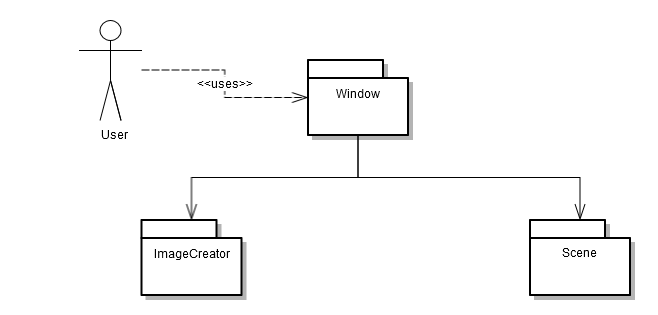
\includegraphics[scale=0.5]{paquetages.png}
		\caption{\label{fig:archi} Diagramme des paquetages en fin de projet \protect \footnotemark}
\end{figure}
\footnotetext{Réalisé grâce au logiciel Gliffy : \url{www.gliffy.com}}


Le paquetage Création tel que présenté dans la figure \ref{fig:creation} n'a pas connu de modifications particulières. En effet, les dépendances entre les différentes classes étaient très importantes pour l'extensibilité du logiciel. Toutefois, de nouvelles classes ont été ajoutées, pour permettre la création des images et des folioscopes.

\begin{figure}[h]
		\centering
                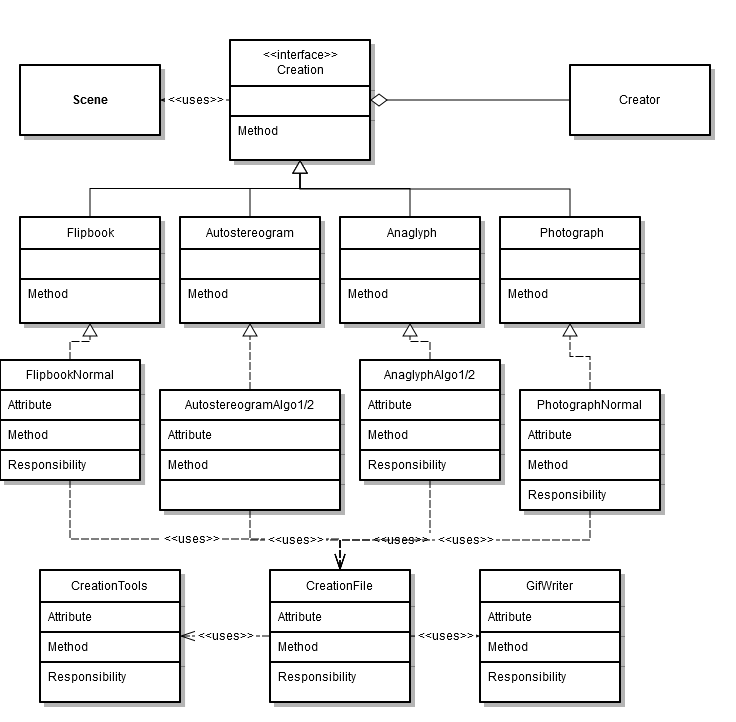
\includegraphics[scale=0.5]{f_creation.png}
		\caption{\label{fig:creation} Paquetage Creation en fin de projet \protect \footnotemark}
\end{figure}
\footnotetext{Réalisé grâce au logiciel Gliffy : \url{www.gliffy.com}}


Le paquetage Interface contient les classes principales permettant la génération des fenêtres du logiciel. Le logiciel QtCreator aura été utilisé pour aider à la génération des ces fichiers sources.

Le paquetage Scene a quant à lui été modifié. Si nous avions initialement prévu que ce soit le Chargeur qui se charge de créer la scène et les objets qui s'y trouvent, c'est finalement la classe Scene en elle-même qui est devenue le point d'entrée du paquetage Scène. Elle se charge ensuite de transférer les informations nécessaires au Chargeur pour qu'il se puisse créer les objets. Le paquetage final de la Scène est présenté dans la figure \ref{fig:scene}.

\begin{figure}[h]
		\centering
                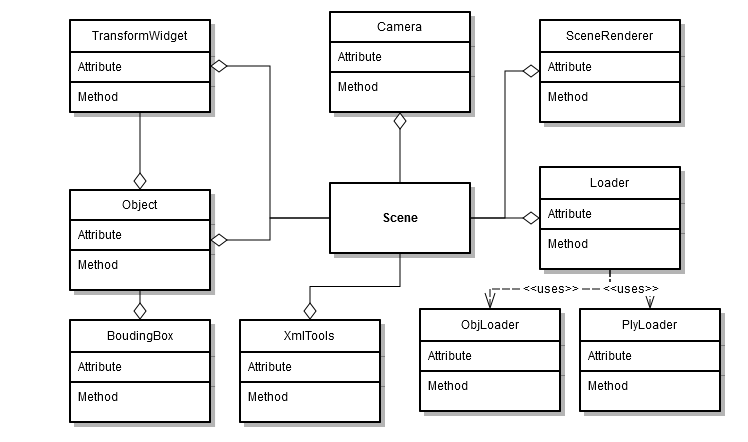
\includegraphics[scale=0.5]{f_scene.png}
		\caption{\label{fig:scene} Paquetage Scene en fin de projet \protect \footnotemark}
\end{figure}
\footnotetext{Réalisé grâce au logiciel Gliffy : \url{www.gliffy.com}}
